% Block decompositions (notebook 42a, Section 5.2).
% (a) a general two-qubit block in KAK form: (u x u) Rxx Ryy Rzz (u x u), u = Rz Ry Rz, 15 angles (kak_block)
% (b) the hardware-efficient block: Ry Rz on each qubit, then a fixed CZ (hardware_efficient_ansatz), 4 angles
% (c) three-qubit block from three two-qubit blocks: 45 angles, while SU(8) has 63 parameters
% (d) four-qubit block from three-, two- and three-qubit blocks (recursion)
\documentclass[tikz,border=6pt]{standalone}
\usepackage{amsmath,amssymb}
\usetikzlibrary{positioning,calc}
\newcommand{\g}[3]{\node[draw, thick, fill=white, minimum width=0.62cm, minimum height=0.5cm, inner sep=1pt, font=\scriptsize] at (#1,#2) {$#3$};}
\newcommand{\blk}[4]{\draw[thick, fill=white] (#1-0.3,-0.75*#2+0.27) rectangle (#1+0.3,-0.75*#3-0.27);
  \node[font=\scriptsize] at (#1,-0.375*#2-0.375*#3) {#4};}
\begin{document}
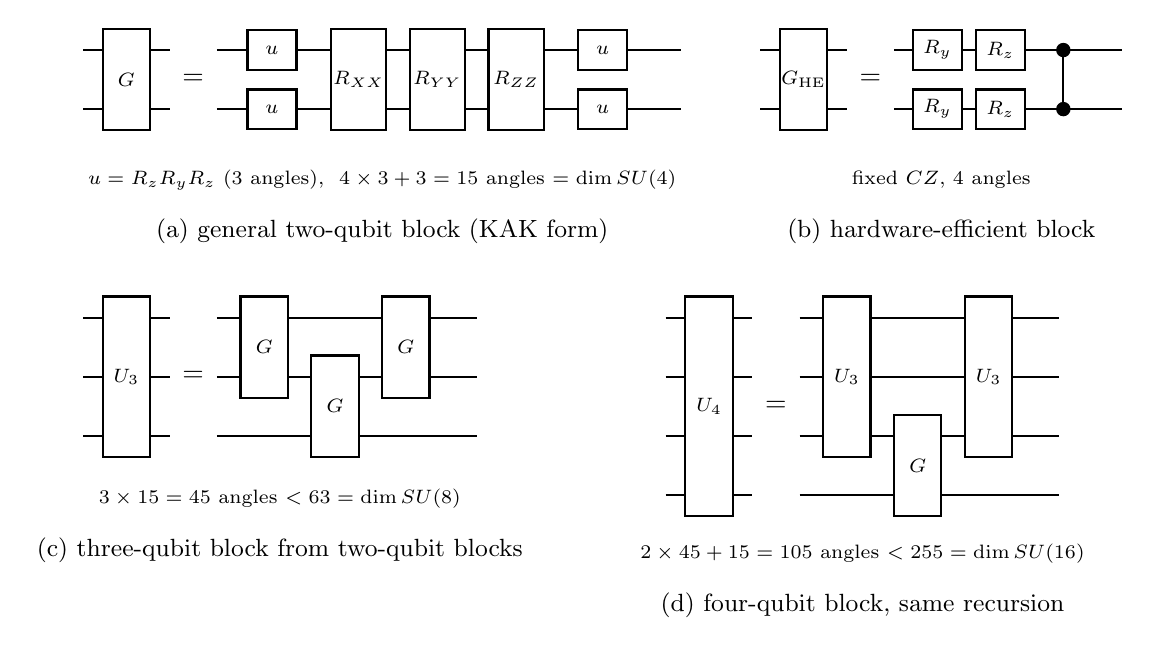
\begin{tikzpicture}
  % ------------------------------------------------------------ (a) KAK block
  \begin{scope}[shift={(0,0)}]
    \foreach \y in {0,-0.75} {\draw[thick] (0,\y) -- (1.1,\y); \draw[thick] (1.7,\y) -- (7.6,\y);}
    \draw[thick, fill=white] (0.25,0.27) rectangle (0.85,-1.02); \node[font=\scriptsize] at (0.55,-0.375) {$G$};
    \node at (1.4,-0.375) {$=$};
    \g{2.4}{0}{u} \g{2.4}{-0.75}{u}
    \draw[thick, fill=white] (3.15,0.27) rectangle (3.85,-1.02); \node[font=\scriptsize] at (3.5,-0.375) {$R_{XX}$};
    \draw[thick, fill=white] (4.15,0.27) rectangle (4.85,-1.02); \node[font=\scriptsize] at (4.5,-0.375) {$R_{YY}$};
    \draw[thick, fill=white] (5.15,0.27) rectangle (5.85,-1.02); \node[font=\scriptsize] at (5.5,-0.375) {$R_{ZZ}$};
    \g{6.6}{0}{u} \g{6.6}{-0.75}{u}
    \node[align=center, font=\scriptsize] at (3.8,-1.65) {$u=R_z R_y R_z$ (3 angles), \ $4\times3+3=15$ angles $=\dim SU(4)$};
    \node[font=\small] at (3.8,-2.3) {(a) general two-qubit block (KAK form)};
  \end{scope}
  % ------------------------------------------------------------ (b) hardware block
  \begin{scope}[shift={(8.6,0)}]
    \foreach \y in {0,-0.75} {\draw[thick] (0,\y) -- (1.1,\y); \draw[thick] (1.7,\y) -- (4.6,\y);}
    \draw[thick, fill=white] (0.25,0.27) rectangle (0.85,-1.02); \node[font=\scriptsize] at (0.55,-0.375) {$G_{\mathrm{HE}}$};
    \node at (1.4,-0.375) {$=$};
    \g{2.25}{0}{R_y} \g{2.25}{-0.75}{R_y}
    \g{3.05}{0}{R_z} \g{3.05}{-0.75}{R_z}
    \draw[thick] (3.85,0) -- (3.85,-0.75);
    \fill (3.85,0) circle (2.6pt); \fill (3.85,-0.75) circle (2.6pt);
    \node[align=center, font=\scriptsize] at (2.3,-1.65) {fixed $CZ$, 4 angles};
    \node[font=\small] at (2.3,-2.3) {(b) hardware-efficient block};
  \end{scope}
  % ------------------------------------------------------------ (c) three-qubit recursion
  \begin{scope}[shift={(0,-3.4)}]
    \foreach \q in {0,1,2} {\draw[thick] (0,-0.75*\q) -- (1.1,-0.75*\q); \draw[thick] (1.7,-0.75*\q) -- (5.0,-0.75*\q);}
    \blk{0.55}{0}{2}{$U_3$}
    \node at (1.4,-0.75) {$=$};
    \blk{2.3}{0}{1}{$G$} \blk{3.2}{1}{2}{$G$} \blk{4.1}{0}{1}{$G$}
    \node[align=center, font=\scriptsize] at (2.5,-2.3) {$3\times15=45$ angles $<63=\dim SU(8)$};
    \node[font=\small] at (2.5,-2.95) {(c) three-qubit block from two-qubit blocks};
  \end{scope}
  % ------------------------------------------------------------ (d) four-qubit recursion
  \begin{scope}[shift={(7.4,-3.4)}]
    \foreach \q in {0,1,2,3} {\draw[thick] (0,-0.75*\q) -- (1.1,-0.75*\q); \draw[thick] (1.7,-0.75*\q) -- (5.0,-0.75*\q);}
    \blk{0.55}{0}{3}{$U_4$}
    \node at (1.4,-1.125) {$=$};
    \blk{2.3}{0}{2}{$U_3$} \blk{3.2}{2}{3}{$G$} \blk{4.1}{0}{2}{$U_3$}
    \node[align=center, font=\scriptsize] at (2.5,-3.0) {$2\times45+15=105$ angles $<255=\dim SU(16)$};
    \node[font=\small] at (2.5,-3.65) {(d) four-qubit block, same recursion};
  \end{scope}
\end{tikzpicture}
\end{document}
